\documentclass[10pt,a4paper]{article}
\usepackage[margin=2.2cm]{geometry}
\usepackage[T1]{fontenc}
\usepackage{lmodern}
\usepackage{microtype}
\usepackage{graphicx}
\usepackage{booktabs}
\usepackage{multirow}
\usepackage{tabularx}
\usepackage{array}
\usepackage{amsmath,amssymb}
\usepackage{siunitx}
\usepackage[table]{xcolor}
\usepackage{caption}
\usepackage{subcaption}
\usepackage{enumitem}
\usepackage{float}
\usepackage[hidelinks]{hyperref}
\usepackage{cleveref}

\definecolor{done}{HTML}{0CA30C}
\definecolor{part}{HTML}{E09A00}
\definecolor{miss}{HTML}{D03B3B}
\definecolor{rowgray}{HTML}{F4F3F0}
\newcommand{\done}{\textcolor{done}{\textbf{Done}}}
\newcommand{\stpart}{\textcolor{part}{\textbf{Partial}}}
\newcommand{\miss}{\textcolor{miss}{\textbf{Not started}}}
\newcommand{\best}[1]{\textbf{#1}}
\newcolumntype{L}{>{\raggedright\arraybackslash}X}
\captionsetup{font=small,labelfont=bf}
\setlist{itemsep=1pt,topsep=3pt}

\title{\textbf{Persistent Object Gaussian Splatting (POGS):\\
Consolidated Progress Report}\\[4pt]
\large Reproduction, real-time tracking benchmark, and a 2D foundation-model substitution study}
\author{[Main author / research coordinator]\\
\small with contributions from the \texttt{pogs-dev} and \texttt{pogs\_v2} workstreams}
\date{13 November 2026}

\begin{document}
\maketitle

\begin{abstract}
\noindent
This report consolidates two parallel workstreams on POGS (Yu \emph{et al.}, ICRA 2025), a method that
tracks rigid objects by optimising per-object poses of a feature-distilled 3D Gaussian Splat
against DINO features and depth. \textbf{Workstream A} (\texttt{pogs-dev}) re-implements the full
scan$\to$train$\to$group$\to$track pipeline with the release's defaults and evaluates it on a
procedurally generated pick-and-place benchmark with exact ground truth (54 offline cases plus a
30\,Hz real-time protocol). Base POGS tracks reliably on slow, unoccluded motion
(100\% ADD-S success) but fails under hand occlusion (34--43\%), large rotations ($\approx$49\% at
90$^\circ$ yaw) and fast motion, and at 25 iterations it runs at only 1.9\,Hz, below the 5\,Hz target.
An SE(3) Kalman prior with a loss check raises overall success from 71\% to 75\%.
\textbf{Workstream B} (\texttt{pogs\_v2}) benchmarks eleven 2D foundation models for the
detection, feature-extraction and feature-alignment roles. The deterministic results (latency, VRAM,
detector IoU) are sound and support the baseline choice of Detic + DINOv2 + CLIP; MobileCLIPv2 is
the only alternative that is faster in its role without a capability loss. The study's tracking
comparison cannot rank the models: only one of four substitutions reached the train/track path
and run-to-run noise (SD 325\,mm) exceeds every between-model difference.
Three objectives (with/without-object splat comparison, tool-perturbation recovery with KL
divergence, and the 80\% in-grasp recovery rate) have not been started. We give a concrete
protocol and plan for each.
\end{abstract}

\tableofcontents
\newpage

%===================================================================
\section{Objectives and scope}
%===================================================================
The project brief defines the work packages in \cref{tab:objectives}. The quantitative targets
are a 5\,Hz tracking frequency, recovery from tool perturbations of up to 30$^\circ$, and an
in-grasp recovery rate of 80\%. The 80\% figure matches the paper's own Table~II result at
30$^\circ$ (40/50 recoveries).

\begin{table}[H]
\centering\small
\caption{Project objectives and their target values.}
\label{tab:objectives}
\begin{tabularx}{\linewidth}{@{}l L l@{}}
\toprule
ID & Objective & Target \\
\midrule
O1 & Object grouping: render splats \emph{with} and \emph{without} a given object and compare,
     to verify that object-specific Gaussians are isolated & qualitative + quantitative \\
O2 & Project structure: Model (detection, features, alignment, POGS), Data (scene generation),
     Metrics (Gaussian, pose) & -- \\
O3 & Tool perturbation recovery: rotate the tool in $\pm5^\circ$ steps, return it to the original
     orientation, compare splats ($x$ vs.\ $y$) and pose; KL divergence & up to 30$^\circ$ \\
O4 & In-grasp tool perturbation recovery rate (same splat + pose comparison) & 80\% \\
O5 & Latency of each 2D foundation model (detection / features / alignment) & per model \\
O6 & Tracking frequency & 5\,Hz \\
O7 & Software environment & Py 3.12, CUDA 13.0, PyTorch 2.14 \\
\bottomrule
\end{tabularx}
\end{table}

%===================================================================
\section{Status summary}
%===================================================================
\begin{figure}[H]
\centering
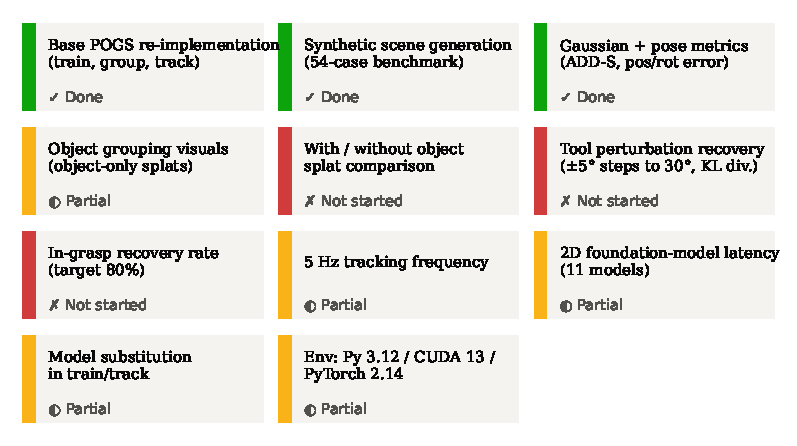
\includegraphics[width=0.92\linewidth]{figures/status_matrix.pdf}
\caption{Status of each work item at the time of writing (13 Nov 2026).}
\label{fig:status}
\end{figure}

\begin{table}[H]
\centering\small
\caption{What has been done and what remains, per objective. A: \texttt{pogs-dev}; B: \texttt{pogs\_v2}.}
\label{tab:status}
\begin{tabularx}{\linewidth}{@{}l l L L@{}}
\toprule
ID & Status & Evidence (done) & Gap (remaining) \\
\midrule
O1 & \stpart & A: HDBSCAN grouping with per-object IoU 0.67--0.98 (\cref{fig:grouping});
     ``object-only'' raw-splat renders in every tracking video (\cref{fig:dash}). &
     No ``scene \emph{minus} object'' render and no quantitative with/without comparison. \\
\rowcolor{rowgray}
O2 & \done & A: \texttt{common/} (model, fields, grouping, tracking, Kalman),
     \texttt{scene\_generator/}, metrics in \texttt{common/evaluate.py}, 17 regression tests;
     B: five model rows with patches. & The two codebases are separate and must be merged into one repository. \\
O3 & \miss & Only pre-audit \texttt{legacy/servoing.py}, whose results were retracted. &
     Protocol, KL-divergence metric and experiment all missing. \\
\rowcolor{rowgray}
O4 & \miss & -- & Needs O3's protocol plus a grasp-perturbation scene. \\
O5 & \stpart & B: fp32/fp16 latency + VRAM for 7 models; Detic and SigLIP2 recovered from logs;
     LocateAnything3D via own harness. & VFM-DETR (no public weights); SigLIP2 standalone; no end-to-end
     per-stage timing inside the tracker. \\
\rowcolor{rowgray}
O6 & \stpart & A: 5\,Hz camera benchmark; tracker 1.9\,Hz (25 it), 4.4\,Hz (10 it), 7.1\,Hz (5 it). &
     No configuration reaches 5\,Hz \emph{and} keeps 25-iteration accuracy. \\
O7 & \stpart & A: PyTorch 2.14 + CUDA 13.0 (on Python 3.14, per \texttt{requirements.txt}). B: torch 2.6/cu118, Python 3.10. & Pin Python 3.12 for A; port B to CUDA 13 / PyTorch 2.14. \\
\bottomrule
\end{tabularx}
\end{table}

\paragraph{Key messages for the supervisor.}
\begin{enumerate}
\item The reproduction (A) is solid and auditable. An internal audit on 2026-11-08 retracted
      every earlier result, and the pipeline was rebuilt to the release's defaults with exact ground truth.
\item Base POGS works when motion is slow and the object is visible. Hand occlusion, unscanned
      faces and speed are the open problems, as the paper itself states in Sec.~VI.
\item The model study (B) gives reliable \emph{latency} numbers but \emph{no} valid accuracy
      ranking. The baseline model set remains the right default.
\item The robotics-specific objectives (O3, O4) and aligning both workstreams on one environment (O7) are the main
      outstanding work.
\end{enumerate}

%===================================================================
\section{Method recap: the POGS pipeline}
%===================================================================
POGS represents a scene as 3D Gaussians, each with a colour, a distilled DINOv2 feature and a
grouping feature trained contrastively from 2D instance masks (Detic). HDBSCAN on the grouping
features yields object clusters. At run time, each tracked object's SE(3) pose is optimised with
Adam so that the rendered DINO features and depth match the current camera frame.
\Cref{tab:pipeline} lists how workstream A matches the authors' release.

\begin{table}[H]
\centering\small
\caption{Implementation fidelity of workstream A against the authors' release.}
\label{tab:pipeline}
\begin{tabularx}{\linewidth}{@{}l L L@{}}
\toprule
Stage & Release & Re-implementation (A) \\
\midrule
Training & splatfacto, 4000 steps; DINO from 100, CLIP + grouping from 2500 & identical; gsplat \texttt{DefaultStrategy} \\
DINO & ViT-S/14, long side 1260, PCA-64, 4-layer MLP head & identical; PCA basis stored in checkpoint \\
Grouping & Detic masks + negative mask, cuML HDBSCAN & simulator instance masks filtered like Detic; sklearn HDBSCAN \\
Selection & interactive click; table cut at $z_\text{table}+1.5$\,cm & geometric selection after the same cut \\
Tracking & ROI, DINO L2 + depth (w=3.7), Adam $4\!\times\!10^{-3}\!\to\!8\!\times\!10^{-4}$, 25 iters & identical \\
\bottomrule
\end{tabularx}
\end{table}

%===================================================================
\section{Synthetic benchmark (Data)}
%===================================================================
A 35-view capture of a floor scene (low table, mug, mustard bottle, soup can, apple, cereal box)
trains a single POGS model (\cref{fig:scan}). A robot gripper picks a target, carries it and places
it on the table: 60 frames at 5\,Hz, 889$\times$500. One factor is changed at a time from the base
condition (mug, 30$^\circ$ yaw, gripper occluder, 1$\times$ speed, 3\,mm depth noise), with
3 random trajectories each (\cref{fig:conditions}, \cref{tab:factors}). Scene v2 uses procedural
materials evaluated in each object's local frame, so textures move with the object.

\begin{figure}[H]
\centering
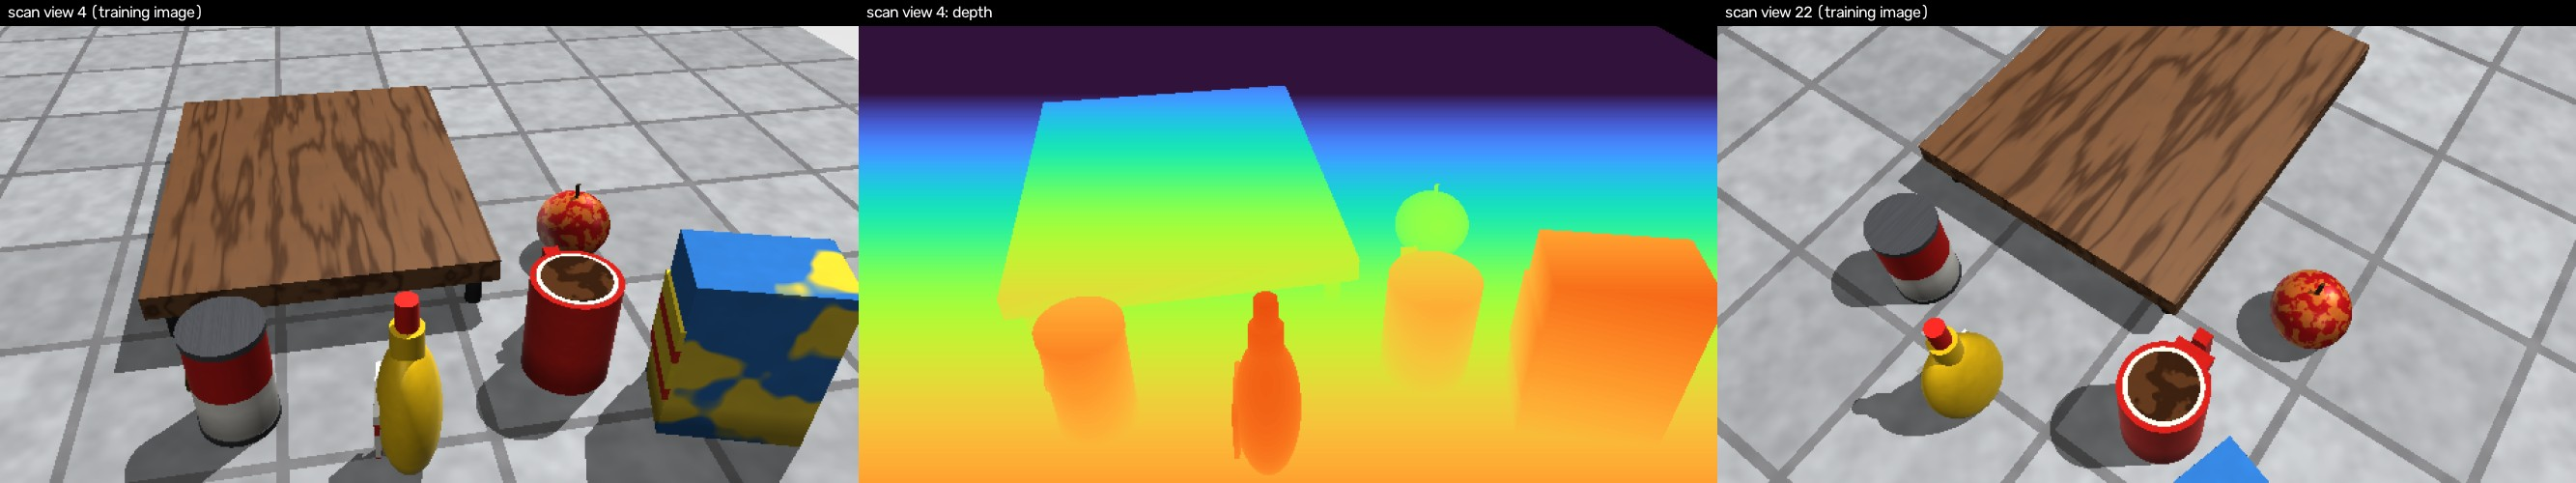
\includegraphics[width=0.85\linewidth]{figures/scan_views.jpg}
\caption{Sample views of the 35-view training capture.}
\label{fig:scan}
\end{figure}

\begin{figure}[H]
\centering
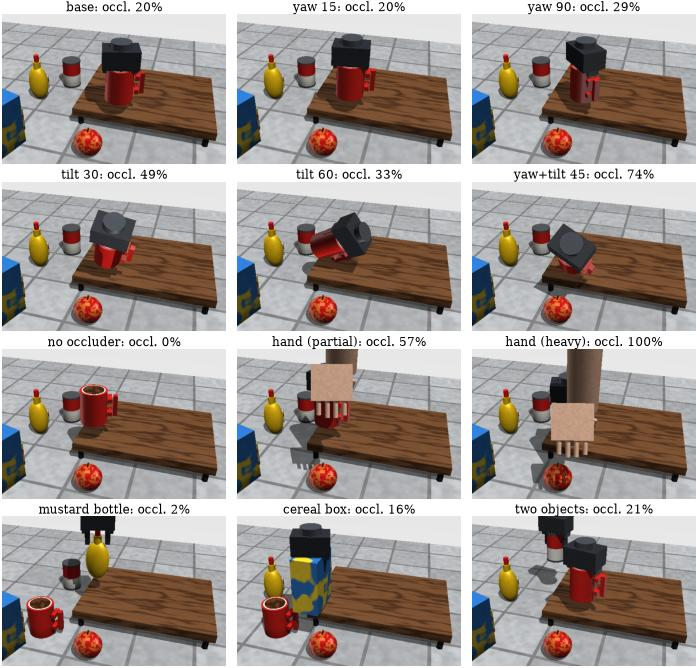
\includegraphics[width=0.78\linewidth]{figures/conditions.jpg}
\caption{The twelve rendered conditions (peak occlusion of the target in each title).}
\label{fig:conditions}
\end{figure}

\begin{table}[H]
\centering\small
\caption{Benchmark factors. Each level has 3 seeds; speed and depth are applied at load time.}
\label{tab:factors}
\begin{tabularx}{\linewidth}{@{}l L L@{}}
\toprule
Factor & Levels & Paper assumption tested \\
\midrule
Rotation & yaw 15/30/90$^\circ$, tilt 30/60$^\circ$, yaw+tilt 45$^\circ$ & unscanned faces (Sec.~III) \\
Speed & frame stride 1/2/4 on base and yaw-90 & ``objects moved slowly'' (Sec.~VI) \\
Occlusion & none / gripper / + hand partial (58\%) / heavy (100\%) & occlusion limitation (Sec.~VI) \\
Depth & clean / 3\,mm / 10\,mm + 5\% holes & reliance on stereo depth \\
Object & mug / mustard bottle / cereal box & shape generality \\
Multi-object & one / two moving & simultaneous tracking \\
\bottomrule
\end{tabularx}
\end{table}

\paragraph{Metrics.}
\emph{ADD-S success} is the fraction of frames whose symmetric average distance is below
10\% of the object diameter. \emph{Lost} is the fraction of frames with position error
$>10$\,cm. Every table includes a \emph{Static} baseline that assumes the object never moves.
The paper's 3\,cm\,/\,5$^\circ$ rule saturates at 10--20\% for all methods because the gripper
tilts the held mug by $\approx$20$^\circ$, so it cannot separate methods.

%===================================================================
\section{Workstream A results: reproduction and tracking}
%===================================================================
\subsection{Reconstruction and object grouping (O1)}
The trained scene has 332k Gaussians, a train-view PSNR of 34.1\,dB and a depth MAE of 0.6\,cm.
HDBSCAN selects all five objects and rejects the floor and table as background (\cref{fig:grouping},
\cref{tab:grouping}).

\begin{figure}[H]
\centering
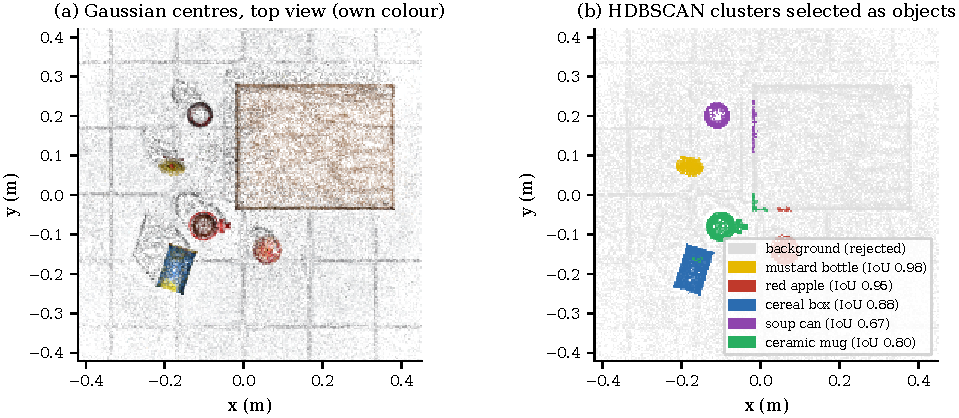
\includegraphics[width=0.9\linewidth]{figures/grouping.pdf}
\caption{Object grouping. (a) Gaussian centres, top view, in their own colour; (b) HDBSCAN clusters selected as objects, with IoU
against ground truth (used only for evaluation).}
\label{fig:grouping}
\end{figure}

\begin{table}[H]
\centering\small
\caption{Grouping quality per object (IoU of the selected cluster against ground-truth Gaussian ownership).}
\label{tab:grouping}
\begin{tabular}{@{}lccccc@{}}
\toprule
& Mustard & Apple & Cereal box & Mug & Soup can \\
\midrule
IoU & \best{0.98} & 0.95 & 0.88 & 0.80 & 0.67 \\
\bottomrule
\end{tabular}
\end{table}

\Cref{fig:dash} shows what O1 asks for in part: the full scene splat beside the splat of the
tracked object alone. The object-only render contains a few stray Gaussians from neighbouring
objects (small yellow and brown blobs), which matches the mug's IoU of 0.80. The missing half of O1
is the complementary ``scene \emph{without} the object'' render together with a quantitative test;
\cref{sec:plan} proposes one.

\begin{figure}[H]
\centering
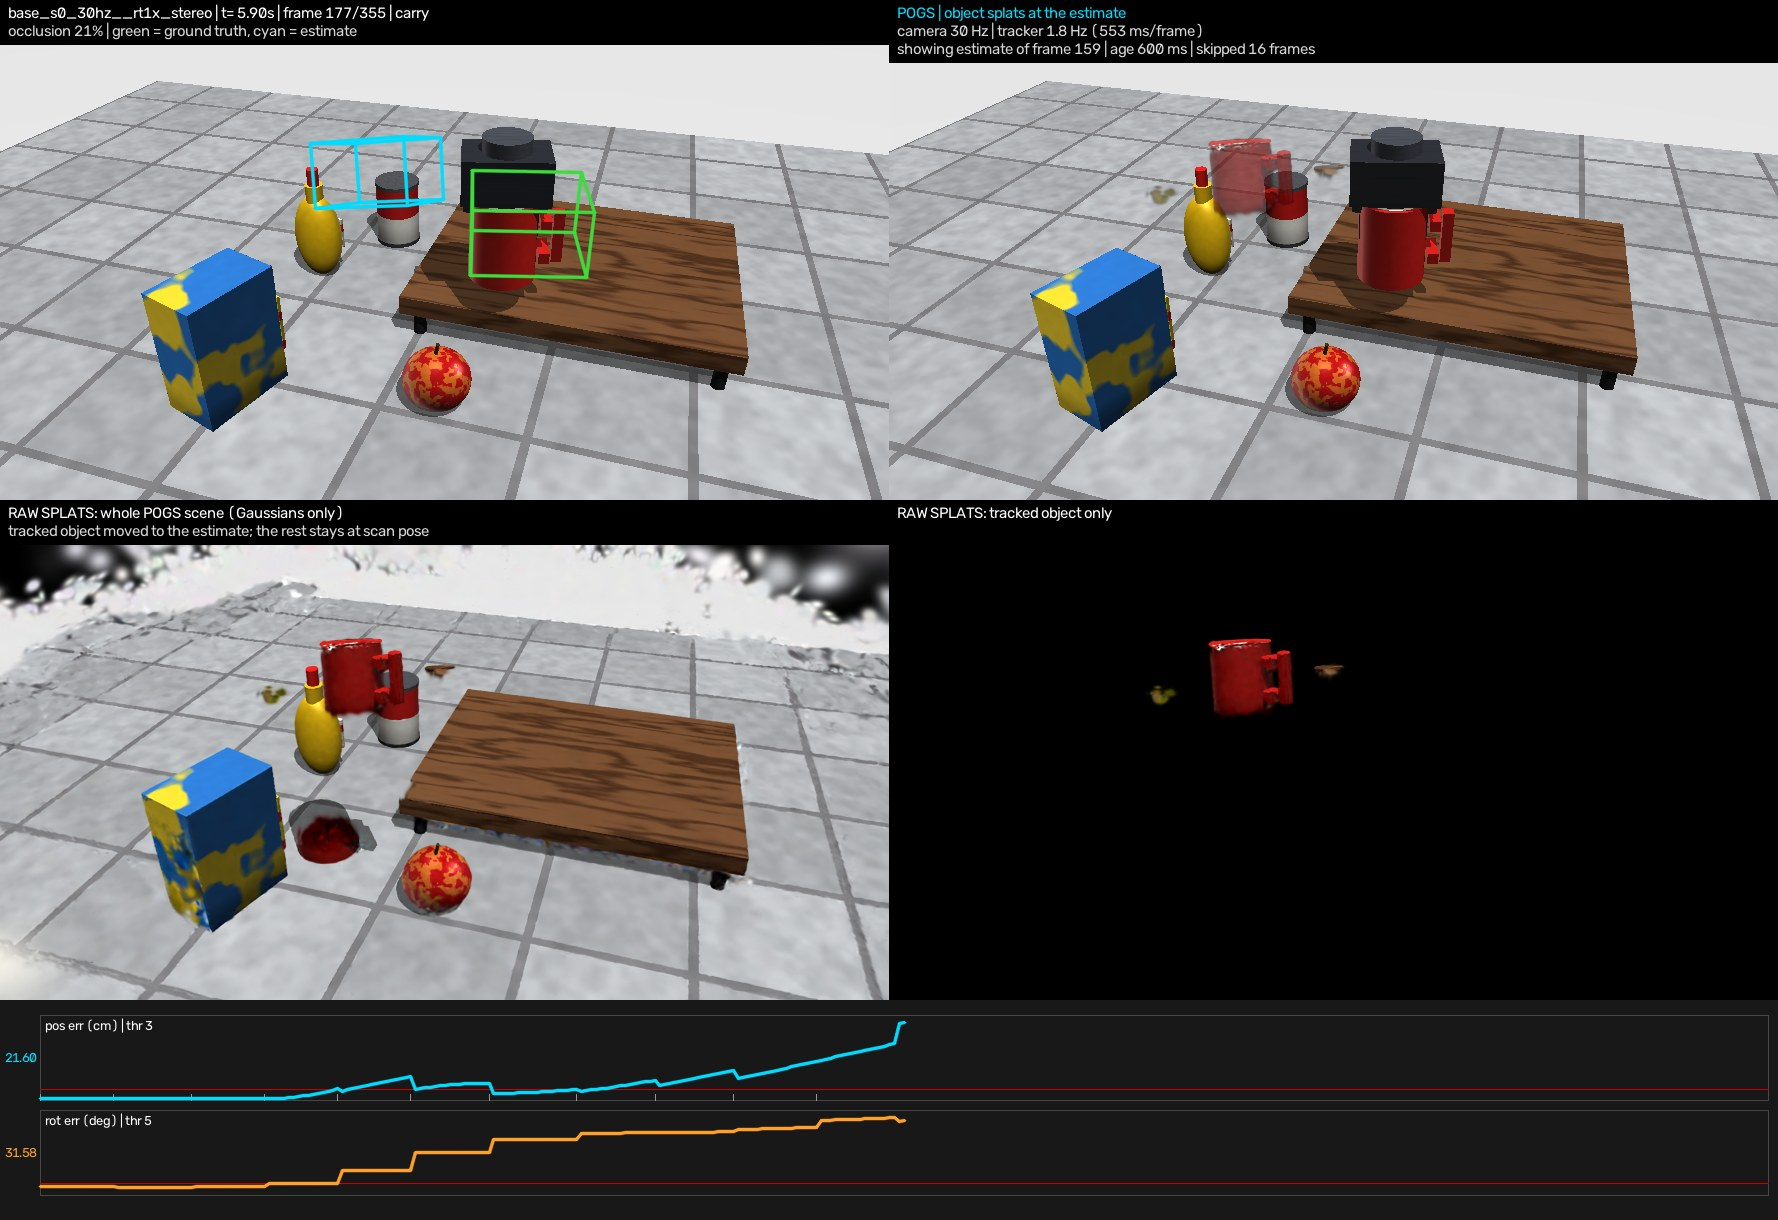
\includegraphics[width=\linewidth]{figures/dash_rt_pogs.jpg}
\caption{Tracking dashboard (base POGS, 30\,Hz camera). Top: camera with ground truth (green) and
estimate (cyan); POGS object splats overlaid at the estimate. Bottom left: raw full-scene splat.
Bottom right: raw splat of the tracked object only. Once the mug moves, most of its Gaussians
leave the scan position, but a dark-red patch remains on the floor there (residual Gaussians
not assigned to the mug's cluster, or baked-in shadow). The with/without test proposed in
\cref{sec:plan} would quantify this.}
\label{fig:dash}
\end{figure}

\subsection{Per-factor tracking accuracy}
\begin{figure}[H]
\centering
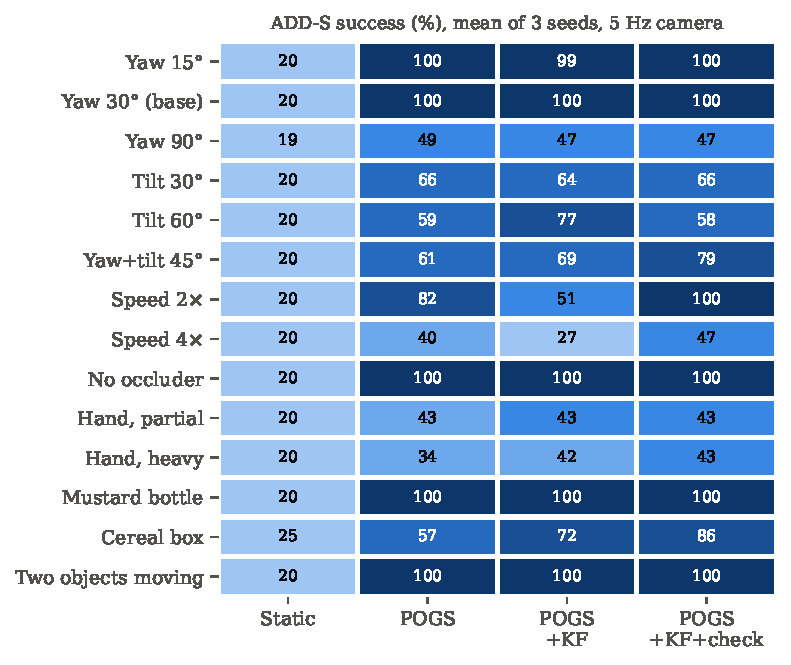
\includegraphics[width=0.62\linewidth]{figures/factor_heatmap.pdf}
\caption{ADD-S success per condition and method (3 seeds, 25 iterations, 5\,Hz camera).}
\label{fig:heatmap}
\end{figure}

\begin{table}[H]
\centering\small
\caption{ADD-S success $\pm$ seed std / lost-frame rate, 25 iterations. Best per row in bold.}
\label{tab:factor}
\begin{tabular}{@{}llcccc@{}}
\toprule
Factor & Level & Static & POGS & POGS + KF & POGS + KF + check \\
\midrule
\multirow{6}{*}{Rotation}
 & yaw 15$^\circ$ & 20 / 73 & \best{100}$\pm$0 / 0 & 99$\pm$1 / 0 & \best{100}$\pm$0 / 0 \\
 & yaw 30$^\circ$ & 20 / 75 & \best{100}$\pm$0 / 0 & \best{100}$\pm$0 / 0 & \best{100}$\pm$0 / 0 \\
 & yaw 90$^\circ$ & 19 / 75 & \best{49}$\pm$15 / 21 & 47$\pm$7 / 10 & 47$\pm$7 / 10 \\
 & tilt 30$^\circ$ & 20 / 74 & \best{66}$\pm$30 / 6 & 64$\pm$32 / 6 & \best{66}$\pm$29 / 7 \\
 & tilt 60$^\circ$ & 20 / 67 & 59$\pm$36 / 37 & \best{77}$\pm$37 / 18 & 58$\pm$36 / 22 \\
 & yaw+tilt 45$^\circ$ & 20 / 73 & 61$\pm$35 / 23 & 69$\pm$33 / 6 & \best{79}$\pm$36 / 7 \\
\midrule
\multirow{2}{*}{Speed}
 & 2$\times$ & 20 / 73 & 82$\pm$31 / 17 & 51$\pm$42 / 4 & \best{100}$\pm$0 / 0 \\
 & 4$\times$ & 20 / 73 & 40$\pm$0 / 60 & 27$\pm$0 / 62 & \best{47}$\pm$7 / 36 \\
\midrule
\multirow{4}{*}{Occlusion}
 & none & 20 / 76 & \best{100}$\pm$0 / 0 & \best{100}$\pm$0 / 0 & \best{100}$\pm$0 / 0 \\
 & gripper & 20 / 75 & \best{100}$\pm$0 / 0 & \best{100}$\pm$0 / 0 & \best{100}$\pm$0 / 0 \\
 & hand, partial & 20 / 76 & \best{43}$\pm$1 / 54 & \best{43}$\pm$0 / 54 & \best{43}$\pm$0 / 54 \\
 & hand, heavy & 20 / 70 & 34$\pm$15 / 52 & 42$\pm$1 / 55 & \best{43}$\pm$0 / 53 \\
\midrule
Depth & 10\,mm + holes & 20 / 75 & 99$\pm$1 / 0 & \best{100}$\pm$0 / 0 & \best{100}$\pm$0 / 0 \\
\midrule
\multirow{2}{*}{Object}
 & mustard & 20 / 73 & \best{100}$\pm$0 / 0 & \best{100}$\pm$0 / 0 & \best{100}$\pm$0 / 0 \\
 & cereal box & 25 / 70 & 57$\pm$13 / 31 & 72$\pm$22 / 14 & \best{86}$\pm$6 / 0 \\
\midrule
Multi-object & two moving & 20 / 69 & \best{100}$\pm$0 / 0 & \best{100}$\pm$0 / 0 & \best{100}$\pm$0 / 0 \\
\bottomrule
\end{tabular}
\end{table}

\paragraph{Findings.}
(i) Slow, visible motion, depth noise up to 10\,mm, the mustard bottle and two simultaneous objects
are at the ceiling, so these conditions do not separate methods.
(ii) Hand occlusion is unsolved by every method ($\le$43\%, $\approx$54\% lost).
(iii) Large rotations and unscanned faces have high seed variance; the Kalman prior lowers the lost
rate (e.g.\ yaw+tilt 45$^\circ$: 23\%$\to$7\%) more than it raises success.
(iv) KF + check gives its clearest wins at 2$\times$ speed (100\% vs.\ 82\%) and on the cereal box
(86\% vs.\ 57\%).

\subsection{Paper ablations}
\begin{table}[H]
\centering\small
\caption{Ablations on the base condition (3 seeds).}
\label{tab:ablation}
\begin{tabular}{@{}lcccc@{}}
\toprule
Method & ADD-S success & Lost & Median pos.\ (cm) & Rot.\ err.\ ($^\circ$) \\
\midrule
Static (no motion) & 20\% & 75\% & 21.99 & 15.0 \\
POGS (DINO + per-frame depth) & \best{100\%} & \best{0\%} & \best{0.78} & 23.1 \\
No depth & 44\% & 17\% & 6.46 & 25.4 \\
No DINO (RGB features) & \best{100\%} & \best{0\%} & 1.09 & \best{22.7} \\
Release default (depth only at init) & 47\% & 23\% & 6.14 & 26.7 \\
\bottomrule
\end{tabular}
\end{table}
Per-frame depth is essential (44\% without it). DINO improves the median error over plain RGB
(0.78 vs.\ 1.09\,cm) but not the success rate on this textured synthetic scene.

\subsection{Tracking frequency and real-time operation (O6)}
In the real-time protocol the camera runs at 30\,Hz. The tracker always takes the newest frame
when it is free and is scored at every camera frame against the pose it has published by then.

\begin{figure}[H]
\centering
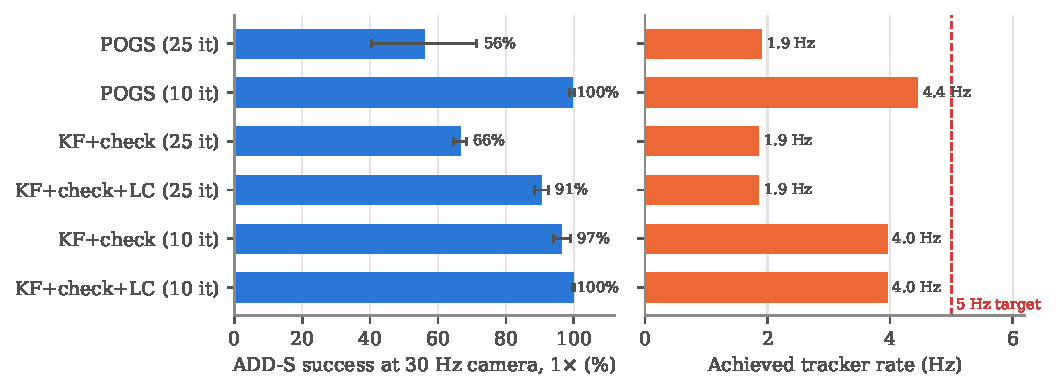
\includegraphics[width=\linewidth]{figures/realtime.pdf}
\caption{Real-time protocol, base trajectory at 1$\times$ (3 seeds). Left: success at the 30\,Hz
camera rate. Right: achieved tracker rate against the 5\,Hz target. LC = latency compensation
(the estimate is extrapolated to ``now'' with the filter velocity).}
\label{fig:rt}
\end{figure}

\begin{table}[H]
\centering\small
\caption{Compute budget over all 54 offline cases. Only the 5-iteration settings exceed 5\,Hz,
and they lose 16--31 points of success.}
\label{tab:budget}
\begin{tabular}{@{}lcccccc@{}}
\toprule
Method & Iters & Rate (Hz) & ADD-S success & Lost & Median pos.\ (cm) & Meets 5\,Hz \\
\midrule
POGS & 25 & 1.8 & 71\% & 22\% & 8.6 & no \\
POGS + KF + check & 25 & 1.7 & \best{75\%} & \best{16\%} & \best{6.4} & no \\
POGS & 10 & 4.1 & 65\% & 30\% & 9.5 & no \\
POGS + KF + check & 10 & 3.6 & 70\% & 24\% & 9.4 & no \\
POGS & 5 & \best{7.1} & 55\% & 36\% & 11.0 & yes \\
POGS + KF + check & 5 & 5.9 & 44\% & 43\% & 15.5 & yes \\
\bottomrule
\end{tabular}
\end{table}

\noindent Base POGS (526\,ms/frame, 1.9\,Hz) publishes poses that are on average 0.8\,s old and
is correct on only 56\% of camera frames. Running 10 iterations (4.4\,Hz), or keeping 25 iterations
and adding Kalman latency compensation, restores 91--100\% at 1$\times$. At 2$\times$ playback every
method fails (20--34\%). \textbf{The 5\,Hz target is therefore not yet met at useful accuracy}; the
gap is roughly a factor of 1.2 at 10 iterations. The latency study (\cref{sec:latency}) suggests
where that time could come from.

%===================================================================
\section{Workstream B results: 2D foundation-model study (O5)}
\label{sec:latency}
%===================================================================
\subsection{Study matrix: intended vs.\ executed}
Five rows were planned to replace the three 2D roles. The training configurations show what
actually ran (\cref{tab:matrix}). Only row 03 substituted a model in the train/track path; rows 01
and 02 are effectively re-runs of the baseline.

\begin{table}[H]
\centering\small
\caption{Planned model combinations and what the training logs show was executed.}
\label{tab:matrix}
\begin{tabularx}{\linewidth}{@{}l L L c@{}}
\toprule
Row & Planned (detection + features + alignment) & Executed in train/track & Real substitution \\
\midrule
00 & Detic + DINOv2 ViT-S/14 + CLIP ViT-B/16 & same (reference) & -- \\
01 & LocateAnything3D [CVPR'26] + dino.txt [CVPR'25] & Detic + DINOv2 + OpenCLIP & no \\
02 & RF-DETR [ICLR'26] + DINOv3 [arXiv'25] + MobileCLIPv2 [TMLR'25] & Detic + DINOv2 + OpenCLIP & no \\
03 & VFM-DETR [NeurIPS'25] + SigLIP2 [DeepMind'25] & Detic + DINOv2 + \textbf{SigLIP2} & alignment only \\
04 & YOLO + DINOv2 + CLIP & latency benchmark only & not run \\
\bottomrule
\end{tabularx}
\end{table}

\subsection{Latency and memory}
All timings were taken on an RTX 4070 (12\,GB) with torch 2.6/cu118, 20 warm-up and 100 timed
iterations, \texttt{cudnn.benchmark} enabled and CUDA synchronisation around every call. Repeat
measurements differ by under 1\,ms.

\begin{table}[H]
\centering\small
\caption{Standalone latency per model on a 1280$\times$720 scene (median over 100 runs). FPS is
the fp16 throughput of the model alone.}
\label{tab:latency}
\begin{tabular}{@{}lllrrrrr@{}}
\toprule
Role & Model & Venue & fp32 (ms) & fp16 (ms) & fp16 p95 & VRAM (MB) & FPS \\
\midrule
Detection & YOLO11x & Ultralytics & 32.1 & 39.8 & 43.2 & 82 & 25 \\
Detection & RF-DETR & ICLR 2026 & 49.3 & 53.7 & 62.9 & 103 & 19 \\
Features & DINOv2 ViT-S/14 & TMLR 2024 & 67.9 & 19.6 & 21.7 & 876 & 51 \\
Features & DINOv3 ViT-B/16 & arXiv 2025 & 89.8 & 34.1 & 37.4 & 1,627 & 29 \\
Feat.+Align. & dino.txt (DINOv2 Meets Text) & CVPR 2025 & 5866.1 & 170.8 & 171.2 & 7,062 & 6 \\
Alignment & CLIP ViT-B/16 & ICML 2021 & 17.0 & 24.0 & 25.8 & 246 & 42 \\
Alignment & MobileCLIPv2 & TMLR 2025 & 13.7 & 20.0 & 22.4 & 258 & 50 \\

\midrule
Detection & Detic (in-pipeline log) & ECCV 2022 & 128--154 & -- & -- & -- & 7 \\
Detection & LocateAnything3D (own harness) & CVPR 2026 & \multicolumn{2}{c}{430--1640 per det.} & -- & 7,938--10,909 & $\le$2 \\
Alignment & SigLIP2-base (in-pipeline) & DeepMind 2025 & \multicolumn{2}{c}{2.4--2.9$\times$ CLIP} & -- & -- & -- \\
Detection & VFM-DETR & NeurIPS 2025 & \multicolumn{5}{c}{no public weights, not measurable} \\
\bottomrule
\end{tabular}
\end{table}

\begin{figure}[H]
\centering
\begin{subfigure}[t]{0.6\linewidth}
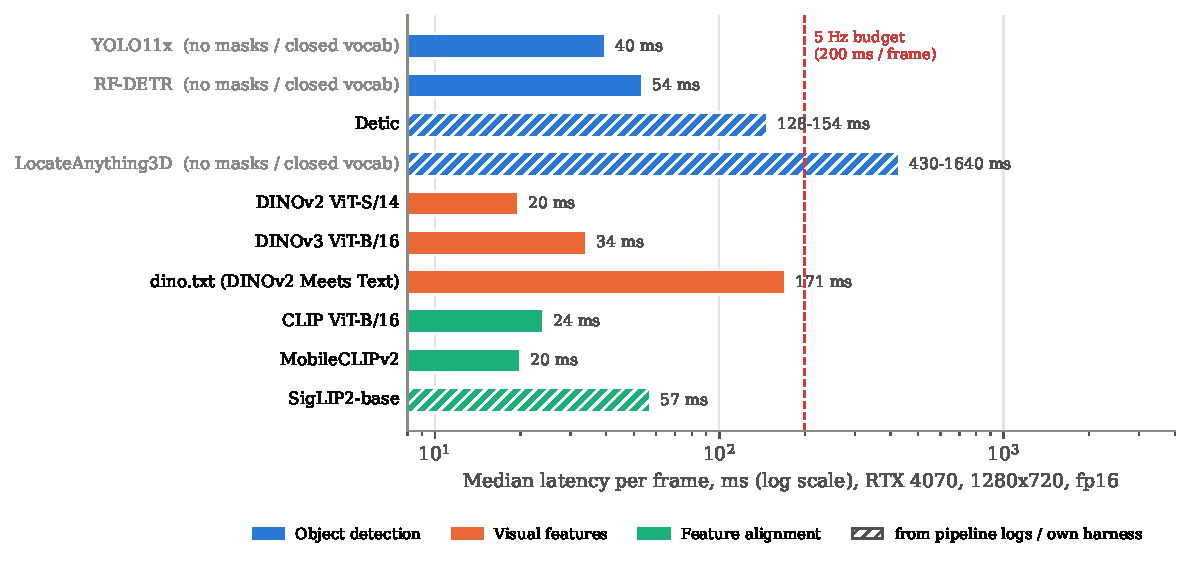
\includegraphics[width=\linewidth]{figures/latency_models.pdf}
\caption{Latency by role. Grey labels: models that cannot serve POGS.}
\end{subfigure}\hfill
\begin{subfigure}[t]{0.38\linewidth}
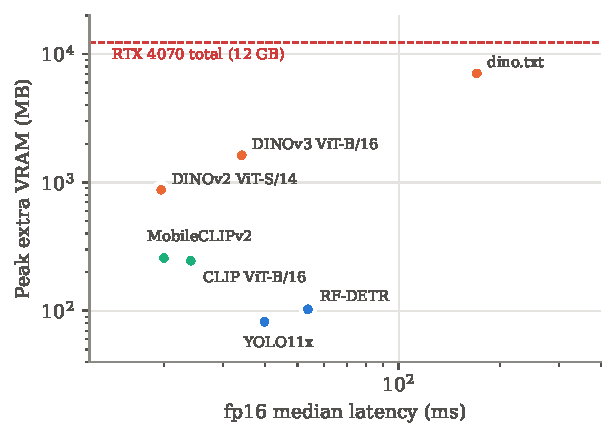
\includegraphics[width=\linewidth]{figures/latency_vram.pdf}
\caption{Latency vs.\ peak VRAM (fp16).}
\end{subfigure}
\caption{Cost of the 2D foundation models. Note the log scales.}
\label{fig:latency}
\end{figure}

\subsection{Capability: the mask contract}
POGS passes an open vocabulary to its detector and needs per-instance 2D masks for its grouping
loss, so a detector that lacks either cannot be used whatever its speed (\cref{tab:capability}).

\begin{table}[H]
\centering\small
\caption{Detector capability against POGS's requirements.}
\label{tab:capability}
\begin{tabular}{@{}lccccl@{}}
\toprule
Detector & Open-vocab & Instance masks & Usable by POGS & Latency & Accuracy \\
\midrule
Detic & \checkmark & \checkmark & \best{yes} & $\approx$148\,ms & IoU 0.617 (real frames) \\
RF-DETR & -- & \checkmark & no & 54\,ms & -- \\
YOLO11x & -- & -- & no & \best{40\,ms} & -- \\
LocateAnything3D & \checkmark & -- (boxes) & no & 0.43--1.64\,s & box IoU 0.46--0.97 \\
VFM-DETR & ? & ? & unknown & -- & no weights \\
\bottomrule
\end{tabular}
\end{table}

\begin{table}[H]
\centering\small
\begin{minipage}[t]{0.46\linewidth}\centering
\caption{Detic on the authors' real ZED capture (14 frames, 120 labels).}
\label{tab:detic}
\begin{tabular}{@{}lr@{}}
\toprule
Metric & Value \\
\midrule
Mean IoU & 0.617 \\
Median IoU & 0.779 \\
Labels IoU $>0.75$ & 58\% \\
Labels IoU $>0.50$ & 66\% \\
Missed (IoU $<0.05$) & 18\% \\
Coverage & 0.975 \\
\bottomrule
\end{tabular}
\end{minipage}\hfill
\begin{minipage}[t]{0.5\linewidth}\centering
\caption{LocateAnything3D first-box IoU per scene family.}
\label{tab:la3d}
\begin{tabular}{@{}lcc@{}}
\toprule
Family & IoU & s/det. \\
\midrule
Pendulum v2 (thick) & 0.96--0.97 & 0.43--0.52 \\
Pendulum v1, 5--10$^\circ$ & 0.91 & 0.44 \\
Pendulum v1, 15--60$^\circ$ & 0.46--0.70 & 0.44--0.57 \\
Pick-place (occluded) & 0.82 & 1.59 \\
Pick-place v2 & 0.69 & 1.64 \\
\bottomrule
\end{tabular}
\end{minipage}
\end{table}

\subsection{Validity of the tracking comparison}
The study's tracking metric is a displacement error. A tracker that reports ``the object never
moved'' scores exactly the mean ground-truth displacement, so any useful tracker must beat that
value. On the pendulum scenes it is not beaten (\cref{fig:noise}), and the same configuration run
with three seeds spans 605\,mm (\cref{tab:seeds}).

\begin{figure}[H]
\centering
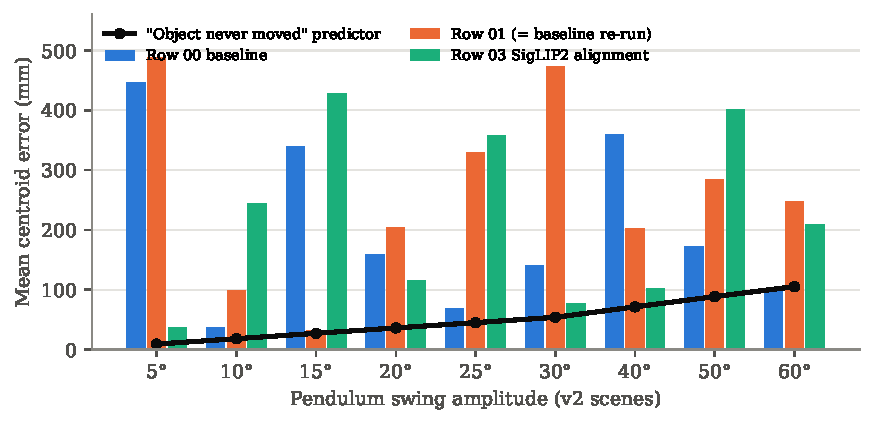
\includegraphics[width=0.85\linewidth]{figures/modelstudy_tracking_noise.pdf}
\caption{Model study, pendulum v2 ladder. All rows lie far above the trivial ``never moved''
predictor (black), and error does not grow with amplitude (Spearman $\rho\in[-0.13,0.13]$), so
these runs do not measure tracking quality.}
\label{fig:noise}
\end{figure}

\begin{table}[H]
\centering\small
\caption{Run-to-run noise against between-model differences (centroid error, mm).}
\label{tab:seeds}
\begin{tabular}{@{}lr@{\hspace{2.5em}}lrr@{}}
\toprule
\multicolumn{2}{@{}l}{Baseline, pick-place, identical config} & \multicolumn{3}{l}{Paired difference on 9 v2 scenes} \\
\cmidrule(r){1-2}\cmidrule(l){3-5}
Seed & Error & Comparison & Mean diff. & $t(8)$ \\
\midrule
42 & 63.4 & Row 01 $-$ Row 00 (same pipeline) & +59.8 & 0.92 \\
13 & 159.8 & Row 03 $-$ Row 00 (SigLIP2) & +16.8 & 0.22 \\
7 & 668.7 & Row 03 $-$ Row 01 & $-$43.0 & $-$0.49 \\
\midrule
SD & \best{325.2} & \multicolumn{3}{l}{none significant ($|t|>2.31$ required)} \\
\bottomrule
\end{tabular}
\end{table}

\paragraph{Verdict per model set.}
\begin{itemize}
\item \textbf{Keep Detic + DINOv2 ViT-S/14 + CLIP ViT-B/16.} It is the only set that satisfies
      the mask contract end to end, and DINOv2-S is the cheapest feature model measured
      (19.6\,ms, 876\,MB).
\item \textbf{Test MobileCLIPv2 next.} It is 1.2$\times$ faster than CLIP at equal VRAM, loads
      through the existing \texttt{open\_clip} call, and has never been wired into train/track.
\item \textbf{Reject} dino.txt (170.8\,ms and 7\,GB at fp16; 11.3\,GB at fp32, 92\% of the GPU),
      DINOv3 (1.7$\times$ slower than DINOv2-S, 1.9$\times$ the VRAM), and the closed-vocabulary or
      box-only detectors.
\item \textbf{SigLIP2} is the only real substitution. It is 2.4--2.9$\times$ slower in its stage
      and its accuracy difference is smaller than the noise floor.
\end{itemize}

%===================================================================
\section{Discussion and threats to validity}
%===================================================================
\begin{itemize}
\item \textbf{Two codebases, two protocols.} A is a clean re-implementation evaluated with ADD-S on
      a 54-case benchmark. B runs the authors' nerfstudio POGS tree with a centroid displacement
      metric on pendulum and pick-place scenes. Their numbers are not directly comparable, and
      their pick-place scenes differ.
\item \textbf{Simulation only.} All tracking results are synthetic. The paper's numbers (2.5--4.1\,cm
      placement error; 48/50 and 40/50 recoveries at 15$^\circ$/30$^\circ$) come from a physical robot
      and must not be compared directly with ours.
\item \textbf{Hardware and environment.} Both workstreams used an RTX 4070. A already runs PyTorch 2.14 /
      CUDA 13.0 (but on Python 3.14); B's latencies were measured on torch 2.6/cu118 and may change
      after porting it to the target stack.
\item \textbf{Seeds.} A uses 3 seeds per condition and reports std. B is mostly $n=1$, and the
      authors' POGS seeds nothing internally (HDBSCAN, feature initialisation, random permutations).
\end{itemize}

%===================================================================
\section{Remaining work and plan}
\label{sec:plan}
%===================================================================
\subsection{Proposed protocols for the open objectives}
\paragraph{O1: with/without-object splat comparison.}
For each selected cluster $\mathcal{G}_k$, render (a) the full scene, (b) the scene with
$\mathcal{G}_k$ removed and (c) $\mathcal{G}_k$ alone from the 35 capture views. Report
(i) the IoU of the rendered alpha of (c) against the ground-truth object mask, (ii) the PSNR of (b)
inside the object mask against a ground-truth render of the scene without the object (which the
simulator can produce), and (iii) the leakage, i.e.\ the rendered opacity of (c) outside the object
mask. A well-grouped object gives high IoU and low leakage, and (b) shows a clean hole with no
residual object colour.

\paragraph{O3: tool perturbation recovery (30$^\circ$) with KL divergence.}
Let $x$ be the object's Gaussians at rest. Rotate the tool in $+5^\circ$ steps to $+30^\circ$
(state $p$), then in $-5^\circ$ steps back to the original orientation (state $y$), tracking every
step. Compare $y$ with $x$ (splats) and the tracked pose with ground truth (pose). As a
distribution-level splat metric we propose the opacity-weighted mean KL divergence between
corresponding Gaussians:
\begin{equation}
D_\text{KL}(x\,\|\,y)=\frac{\sum_i \alpha_i\,\mathrm{KL}\!\left(\mathcal{N}(\mu_i^x,\Sigma_i^x)\,\|\,
\mathcal{N}(\mu_i^y,\Sigma_i^y)\right)}{\sum_i\alpha_i},
\end{equation}
\begin{equation}
\mathrm{KL}(\mathcal{N}_0\|\mathcal{N}_1)=\tfrac12\Big[\operatorname{tr}(\Sigma_1^{-1}\Sigma_0)
+(\mu_1-\mu_0)^\top\Sigma_1^{-1}(\mu_1-\mu_0)-3+\ln\tfrac{\det\Sigma_1}{\det\Sigma_0}\Big].
\end{equation}
Because POGS moves each group rigidly, correspondence is exact (same index $i$), and $D_\text{KL}=0$
if and only if the object returns exactly to its original pose. Report $D_\text{KL}$, position and
rotation error at each step, and the largest step angle at which tracking still recovers.

\paragraph{O4: in-grasp recovery rate (80\%).}
Repeat O3 with the tool held in the gripper, perturbing it by $\pm15^\circ$ and $\pm30^\circ$
(clockwise and counter-clockwise) over $N=50$ trials per level, as in the paper's Table~II.
A trial succeeds if, after the perturbation, the tracked tool tip is within 3\,cm and 5$^\circ$ of
ground truth within a fixed number of frames. Report the recovery rate with a Wilson 95\% interval.
The target is $\ge80\%$ at 30$^\circ$.

\subsection{Work plan}
\begin{table}[H]
\centering\small
\caption{Prioritised remaining work.}
\label{tab:plan}
\begin{tabularx}{\linewidth}{@{}c l L c c@{}}
\toprule
\# & Item & Action & Obj. & Effort \\
\midrule
1 & Repository merge & Import A as the core library; add B's latency harness and patches under \texttt{model/}; one environment & O2 & 2--3 d \\
2 & Environment port & Pin Python 3.12 for A and re-run the 17 tests; port B from torch 2.6/cu118 to PyTorch 2.14 / CUDA 13.0 & O7 & 2 d \\
3 & With/without splats & Render (a)/(b)/(c), IoU, leakage, PSNR for all 5 objects & O1 & 1 d \\
4 & Perturbation scene & Tool object + in-gripper rotation trajectories ($\pm5^\circ$ steps, $\pm15/30^\circ$) in the generator & O3/O4 & 2--3 d \\
5 & KL metric & Implement $D_\text{KL}$ in \texttt{metrics/gaussian}; unit test (identity $\Rightarrow0$) & O3 & 0.5 d \\
6 & Recovery experiments & 50 trials $\times$ 4 settings; recovery rate with CI & O3/O4 & 2 d GPU \\
7 & 5\,Hz tracker & Profile per-stage time; try MobileCLIPv2, fp16 DINO, 10--15 iters + KF latency comp. & O6 & 2 d \\
8 & Model study re-run & Wire MobileCLIPv2 into train/track; 5 seeds on pick-place; ADD-S metric from A & O5 & 1.5 d GPU \\
\bottomrule
\end{tabularx}
\end{table}

\subsection{Structure of the consolidated repository}
Both workstreams are merged into \texttt{github.com/Shakhoyat/POGS-Final}. Workstream A is
imported with its full commit history; workstream B (not under version control) is imported as
code plus its byte-identical results archive. Items marked \emph{new} are still to be written.
\begin{verbatim}
POGS-Final/
  model/  pogs/               core POGS library (A)
          foundation_study/   detection / features / alignment study (B)
  data/   scene_generator/    synthetic benchmark (A); + perturbation scenes (new)
  metrics/                    gaussian (KL, IoU, leakage) + pose (recovery rate) (new)
  experiments/                v1_base_pogs, v2_kalman_pogs, v3, realtime (A)
  tests/                      17 regression tests (A)
  report/ reproduction/       A's detailed report
          supervisor/         this document + make_figures.py
  docs/  third_party/  legacy/  tools/
\end{verbatim}

%===================================================================
\section{Conclusion}
%===================================================================
The POGS reproduction is complete and validated on a synthetic benchmark with exact ground truth.
It shows that POGS is accurate for slow, visible manipulation and identifies occlusion, unscanned
faces, speed and the 1.9\,Hz tracker rate as its limits; a Kalman prior with a loss check partly
mitigates the last three. The foundation-model study gives reliable cost measurements that confirm
the baseline models and single out MobileCLIPv2 as the one promising swap, but its accuracy
comparison must be repeated with multiple seeds on a valid scene. The next phase merges both
codebases, ports them to the target environment, and runs the three robotics experiments (O1, O3,
O4) under the protocols defined above.

\appendix
\section{Reproducibility}
\begin{itemize}
\item Figures and the latency table are regenerated from cached results by
      \texttt{python report/supervisor/make\_figures.py} (CPU only).
\item Workstream A: \texttt{data\_results/*/summary.csv}; runs cached in
      \texttt{data\_results/benchmark\_runs/}; detailed report in \texttt{report/reproduction/main.pdf}.
\item Workstream B: \texttt{model/foundation\_study/artefacts/**/\{latency,tracking\}.json};
      analysis in \texttt{model/foundation\_study/COMPARISON\_STUDY.md}.
\item Hardware: NVIDIA RTX 4070 (12\,GB).
\end{itemize}

\end{document}
